\section{Analisi dei dati}\label{sec:analisi}
\normalsize
In questa sezione saranno analizzati i dati di SkillCraftI per cercare di capire la struttura dei dati e correggere eventuali problemi che il dataset potrebbe avere. Per fare questo saranno usate le librerie Python Matplotlib e Seaborn, che permettono di graficare i dati per renderli più leggibili e interpretabili.   
\subsection{Bilanciamento del dataset}\label{ssec:bilanciamento}
\normalsize
\par
Le leghe di starcraft sono per loro natura sbilanciati, dal sito Liquipedia \cite{liquipedia}, un'enciclopedia online a tema videogiochi, si può leggere come sono strutturare le leghe del gioco e gli obbiettivi che si sono posti gli sviluppatori quando le hanno create. \\*\\*
La distribuzione a cui puntavano gli sviluppatori è come segue:
\begin{itemize}
	\item Grand Master 1000 giocatori
	\item Master 2\%
	\item Diamante 18\%
	\item Platino 20\%
	\item Oro 20\%
	\item Argento 20\% 
	\item Bronzo 20\%
\end{itemize}

Nella realtà le cifre sono destinate ad essere leggermente diverse, ma la proporzione è a grandi line corretta. \\*
In più oltre, alle leghe del gioco, nel data set possiamo trovare anche i giocatori professionisti. Questa ulteriore divisione è stata aggiunta perché, anche se i grand master possono essere considerati un elite tra i giocatori, il divario le loro capacità e quelle dei professionisti è considerevole. 
Nel database Skillcraft invece le proporzioni sono indicate nel grafico a seguire\\*
\begin{center}
	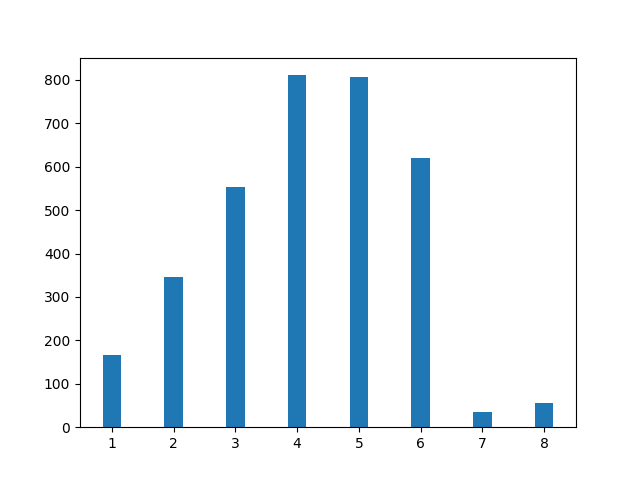
\includegraphics[scale=0.8]{../figures/sbilanciamento.PNG}
\end{center}
\par
Come previsto il dataset è sbilanciato, questo comporta che bisognerà prestare attenzione a come vengono raggruppati i sample durante l’addestramento dei modelli e lo splitting. Oltre a questo, l’unica altra anomalia che è possibile individuare è che al contrario delle aspettative ci sono più professionisti che Grand Master, questo non è rispecchiato nella realtà ed è dovuto al modo in cui sono stati campionati i dati, ma ai fini della classificazione non dovrebbe creare grossi problemi.

\subsection{Elementi nulli}\label{ssec:nulli}
\normalsize
\par
Per la buona riuscita dell’addestramento è necessario rimuovere gli elementi nulli e il nostro dataset ne ha alcuni, ora cercheremo di capire quanti sono e come sono distribuiti per trovare una soluzione al problema.\\*\\*
Il grafico sotto rappresenta il numero totale di elementi nulli per ogni rank divisi per la feature a cui appartengono.\\*
\begin{center}
	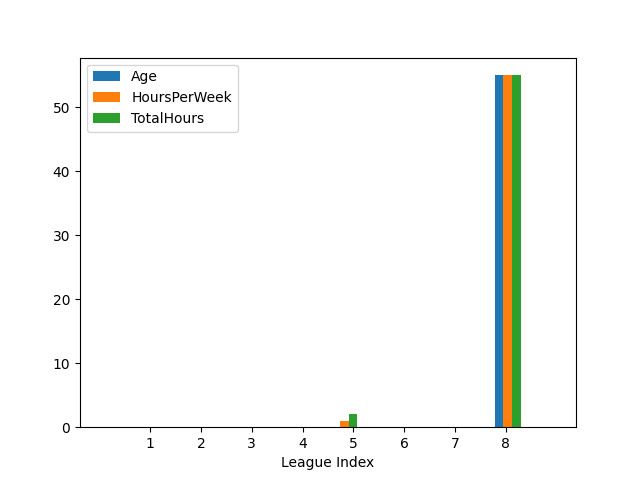
\includegraphics[scale=0.9]{../figures/Nan_distribuzione.PNG}
\end{center}
\par
Dal grafico si può vedere che gli elementi nulli sono concentrati in 3 features che rappresentano: Età, ore di gioco settimanali e ore di gioco totali, in più la maggior parte è nella lega 8, ovvero i professionisti. \\*\\*
Esistono diverse soluzioni per gestire gli elementi nulli di un dataset, si possono eliminare le righe che ne contengono uno, ma controllando i dati dei professionisti si può notare che le tre colonne identificate prima sono tutte nulle in questa lega, di conseguenza eliminare le righe con elementi nulli vorrebbe dire perdere completamente i dati sui professionisti.\\*\\*
Un'altra alternativa è quella di riempire i dati nulli con un valore che potrebbe estimarli, come la media degli altri valori di quella feature in quella lega, ma come visto prima non ci sono altri valori su cui costruire la stima e di conseguenza questa strada è impraticabile.\\*\\*
L’unica alternativa rimasta è eliminare le colonne con i valori nulli, ma come possiamo misurare l'effetto che questa decisione avrà sulla classificazione? Con una mappa di correlazione!\\*
La mappa di correlazione rappresenta la relazione lineare tra i suoi elementi, da essa è possibile capire quanto due feature sono legate tra di loro e con la classe che vogliamo predire.\\*
\begin{figure}[htp]
\makebox[\textwidth][c]{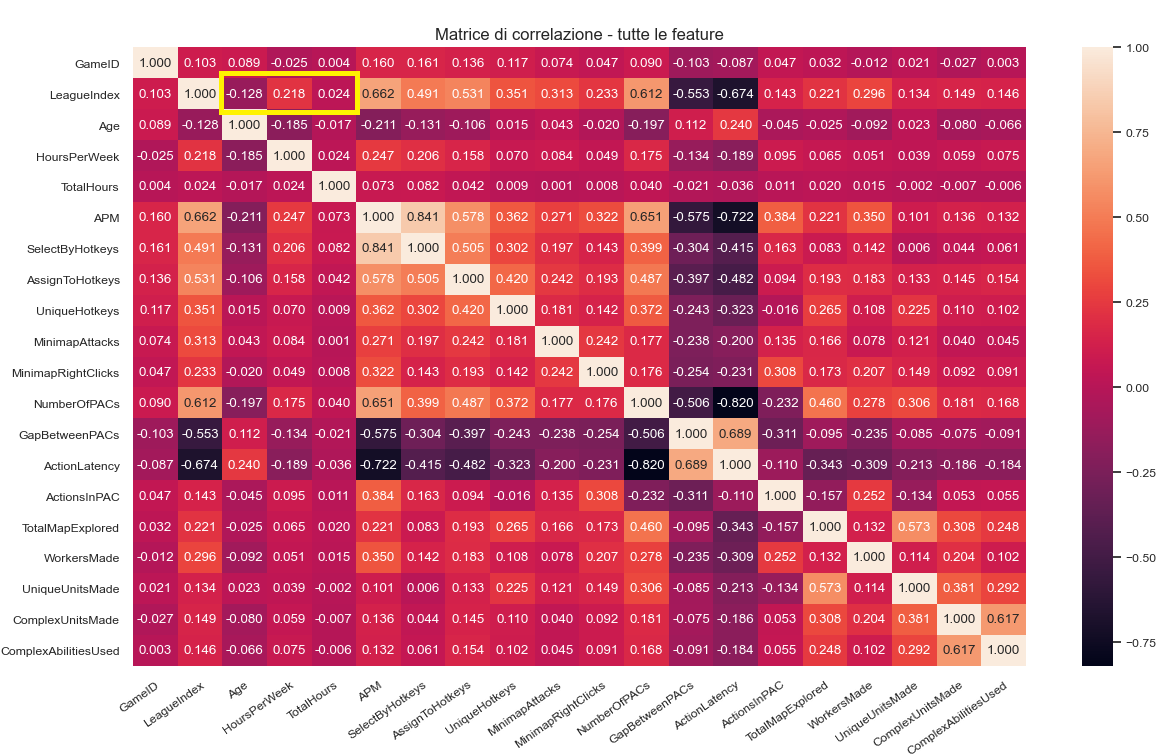
\includegraphics[scale=0.6]{../figures/correlation totale corretta.PNG}}
\end{figure}
\par
I valori evidenziati in giallo sono gli indici di correlazione delle feature con valori nulli, fortunatamente sono tendenzialmente bassi, quindi togliendoli non andremo ad influire sulla classificazione, ma potremmo addirittura migliorare le prestazioni di certi algoritmi di classificazione.
\clearpage

\subsection{Relazioni tra le feature}\label{ssec:relazioni}
\normalsize
\par
Ora è il momento di controllare come sono fatte le feature, che relazioni hanno tra di loro e in particolare con il target da classificare.\\*\\*
Per farlo useremo due grafici principalmente il pairplot e la matrice di correlazione vista prima, il primo serve a definire il tipo di relazione, mentre la seconda da un’indicazione più quantitativa della relazione. \\*\\*
Il pairplot è essere usato per guardare le relazioni tra tutte le feature, ma nel nostro caso è sconveniente vista la grossa numerosità delle feature, i grafici verrebbero troppo piccoli di disordinati per essere utili. Quindi ho deciso si fare un pairplot con solo le relazioni delle feature con il nostro target, ovvero l’indice della lega.
\begin{figure}[htp]
\makebox[\textwidth][c]{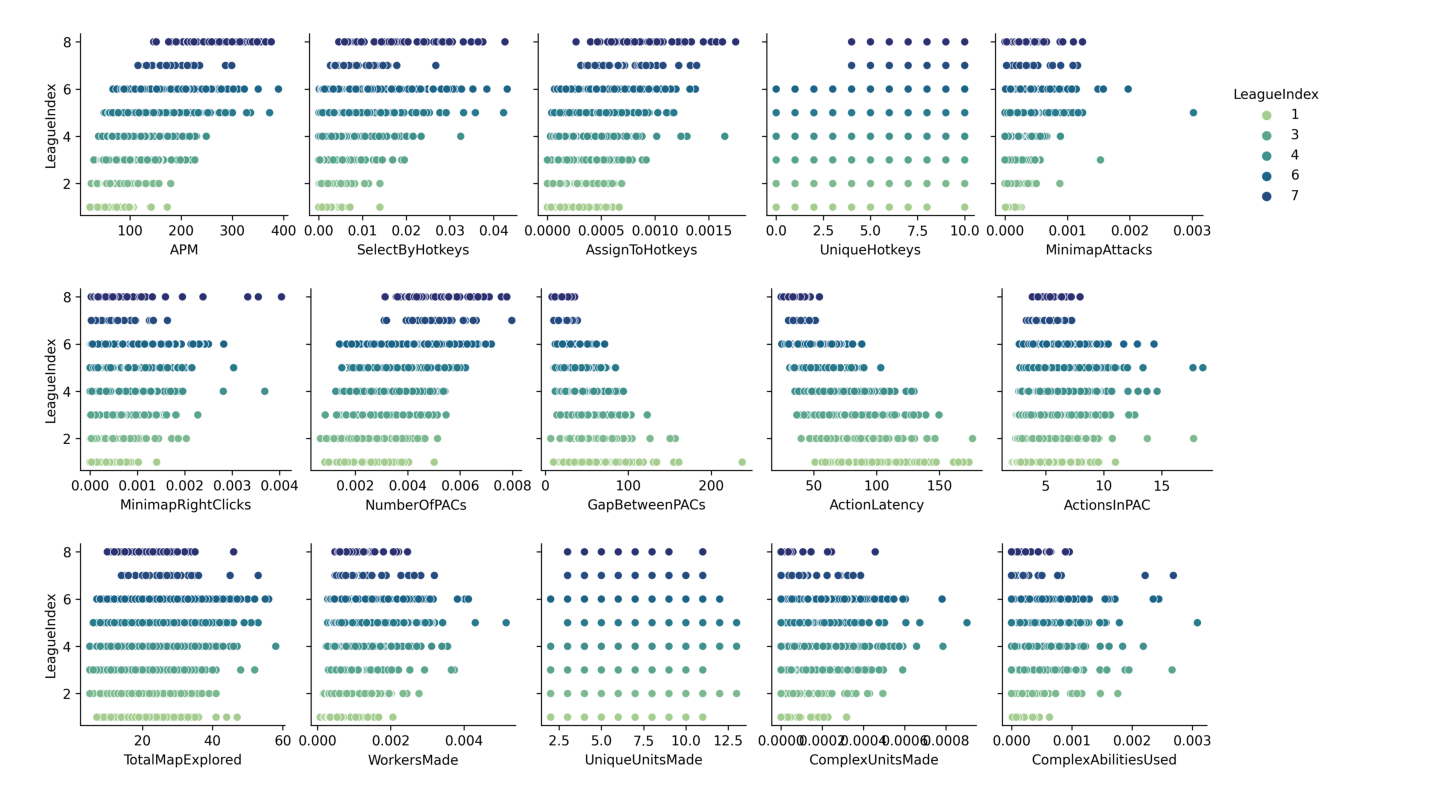
\includegraphics[scale=0.5]{../figures/pairplot_features_target.PNG}}
\end{figure}
\par
Le cose che possiamo notare dai due grafici sono principalmente due, la prima è che guardando il pairplot possiamo notare che, alcune features hanno dei pattern nella loro relazione con il target, in particolare l'APM e l'ActionLatency, le due feature con la correlazione maggiore, sembrano seguire un andamento vagamente lineare.\\*
 Per quanto riguarda la mappa di correlazione invece possiamo notare che alcune features hanno una relazione forte tra di loro che è un indice di collinearità e multicollinearità, questi fenomeni sono abbastanza pericolosi perché rendono i modelli suscettibili al rumore delle feature. \\*\\*
Analizzando questo caso a fondo però è possibile rendersi conto che queste feature, sebbene collegate, non sono l’una la diretta conseguenza dell’altra. Prendendo ad esempio le APM e il numero di selezioni fatte con tasti personalizzati, l’usare dei tasti personalizzati, se fatto male può portare anche al calo degli APM dovuto al tempo necessario per correggre gli errori, l’abilità di fare queste operazioni correttamente è un buon indice della qualità di un giocatore. \\*
Visto che anche gli altri casi sono simili a questo, ovvero dove c’è una dipendenza, ma penso che la relazione che sussiste tra di loro sia significativa alla classificazione, ho deciso di lasciare tutte le feature per ora. \\*\\*
Per essere sicuro però ho deciso di inserire tra i modelli il random forest classifier, che è un classificatore che soffre poco a causa della collinearità/multicollinearità, e usarlo un po' come cartina torna sole, se le sue prestazioni finali saranno di molto maggiori rispetto a quelle degli altri modelli sarà necessario tornare indietro e selezionare meglio le feature.
